\section{{{\fontsize{17}{21}\selectfont \textbf{Objective}}}}
\setlength{\columnsep}{1.5cm}
\begin{figure}[h]
  \centering
  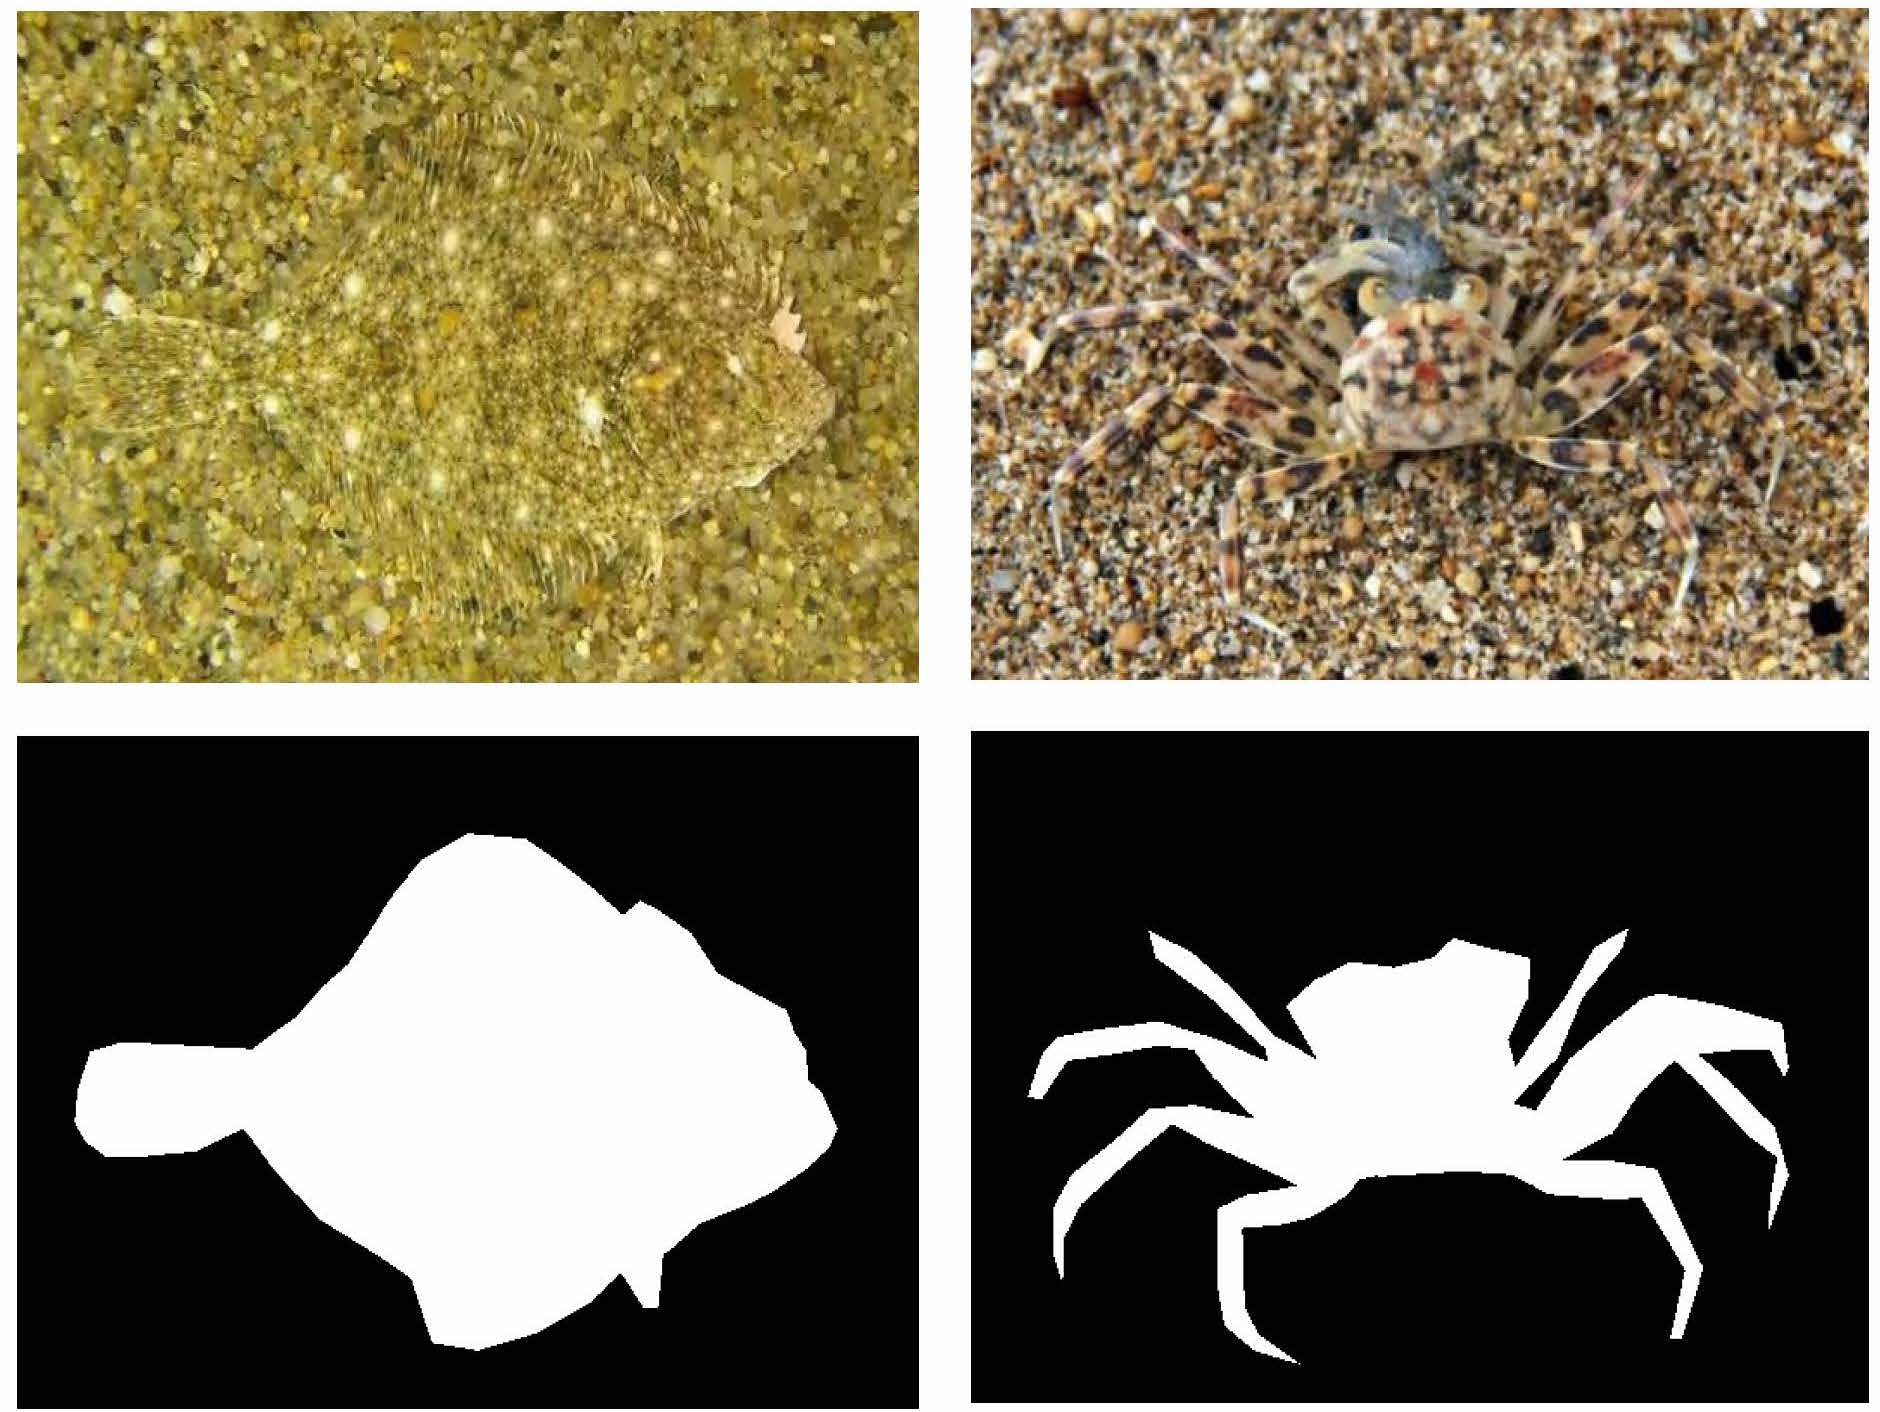
\includegraphics[width=0.8\textwidth]{sections/LBP/camouflaged_object_zIElgp0.jpg}
  \caption{Objective of our project(To create binary mask image to detect camouflage}
  \label{fig:figure_label}
\end{figure}

\begin{multicols}{2}
\ The primary objective of our project is to develop an effective and efficient camouflage detection system based on the SINet architecture. \\
We aim to develop a model which can detect both RGB and multi-spectral images. For that we aim to train create the model using SINet architecture and train it on RGB Camouflage Dataset as it is easy to get RGB dataset with large number of images. After training the network on RGB dataset we aim to train it on multispectral data, and for that we are required to perform data fusion on drone data to obtain the multispectral dataset.
\end{multicols}

\vspace{0.5cm}
{\color{gray}\hrule}
\vspace{0.5cm}